\documentclass[../sparc.tex]{subfiles}
\graphicspath{{\subfix{../images/}}}
\begin{document}

%%%%%%%%%%%%%%%%%%%%%%%%%%%%%%%%%%%%%%%%%%%%%%%%%%%%%%%%%%%%%%%%%%%%%%%%%%%%%%%%
\section{Полутона, диезы и бемоли}

Мы с вами всю эту главу говорим, что нот в октаве семь, и суммарно звуков 63
штуки, если считать по всем октавам. Но это не совсем точно -- на самом деле
звуков в октаве не семь, а двенадцать!

Вот так сюрприз. Откуда берутся дополнительные пять звуков? Оказывается, что в
музыке есть так называемые \emph{полутона}, которые позволяют разнообразить
музыку новыми звуками.

Нагляднее всего эти скрытные звуки легче всего увидеть на клавиатуре пианино
(см. рис. \ref{fig:piano-keyboard}.)

\begin{figure}[ht]
  \centering
  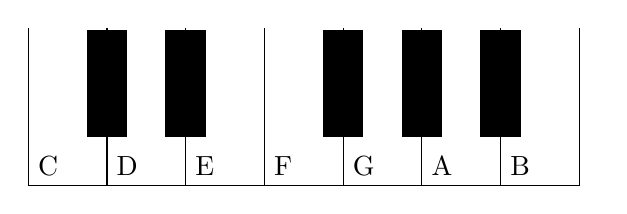
\begin{tikzpicture}
    \draw (0, 0) -- (7, 0);
    \foreach \x/\note in {0/C, 1/D, 2/E, 3/F, 4/G, 5/A, 6/B, 7/} {
      \draw (\x, 0) -- (\x, 2) -- (\x, 0) node[anchor=south west] {\note};
    };
    \foreach \x in {1, 2, 4, 5, 6} {
      \node[
        rectangle,
        draw,
        fill=black,
        minimum width=0.5cm,
        minimum height=1.35cm
      ] (r) at (\x, 1.30) {};
    };
  \end{tikzpicture}
  \label{fig:piano-keyboard}
  \caption{Одна октава на клавиатуре пианино.}
\end{figure}

Видно, что между парами нот ``C''--``D'', ``D''--``E'', ``F''--``G'',
``G''--``A'', ``A''--``B'' находятся чёрные клавиши. Если мы посчитаем, сколько
всего клавиш в одной октаве, то получим двенадцать штук -- двенадцать звуков.

Объясняется это тем, что между двумя соседними клавишами \emph{расстояние в один
полутон}, если представить частотный диапазон октавы как некий отрезок.
Большинство пар нот имеют друг от друга достаточное расстояние, чтобы туда,
ровно посерёдке, добавить ещё одну клавишу (исключение составляют пары
``B''--``C'', ``E''--``F''.)

Каких-то особых закорючек для этих дополнительных звуков в музыке не
применяется, однако есть ``модификаторы'' для основных семи нот, поднимающих или
понижающих их частоту на полутон.

Для того, чтобы например получить частоту клавиши между парой ``C''--``D'',
можно поднять частоту ``C'' на пол-тона, либо понизить частоту ``D'' на те же
пол-тона.

Модификатор, повышающий частоту ноты на пол-тона называется \emph{диезом}, тогда
как аналогичный модификатор, понижающий частоту на пол-тона, называется
\emph{бемолем}.

\index{Музыка!Диез}
Ноты с модификатором ``Диез'' помечаются решёткой (``\#''), стоящей перед нотой
-- например, на рис. \ref{fig:lilypond-f4-sharp} изображена ``Фа Диез''
четвёртой октавы.

\begin{figure}[ht]
  \caption{``Фа Диез'' четвёртой октавы.}
  \centering
  \begin{lilypond}
    \relative c' {
      \numericTimeSignature
      \time 4/4
      fis4
    }
  \end{lilypond}
  \label{fig:lilypond-f4-sharp}
\end{figure}

Чтобы высчитать частоту ``F4\#'', надо найти среднее арифметическое для частот
ноты ``F4'' и следующей перед ней ноты ``G4'' (см. формулу
\ref{equation:f-sharp-calculation}.)

\begin{equation}
  \frac{\mbox{F4} + \mbox{G4}}{2} = \mbox{F4\#}
  \label{equation:f-sharp-calculation}
\end{equation}

Программно вычислить ``F4\#'' не составляет труда, как показано в коде ниже.
Заметьте, что мы обозначили получившуюся частоту, как \texttt{f4s}, так как ``Фа
Диез'' по-английски пишется, как ``Fa Sharp'', и мы используем букву ``s'' из
слова ``sharp'' после ноты для краткости.

\begin{listing}[ht]
  \begin{minted}{cpp}
    const float f4  = 349.230;
    const float g4  = 392.000;
    const float f4s = (f4 + g4) / 2; // F4 Диез
  \end{minted}
  \label{listing:music-f4-sharp}
  \caption{Вычисление ``диеза'' для ноты.}
\end{listing}

Подобный подход работает и с другими нотами.

Кстати, для тех нот, после которых нет чёрной клавиши (``B'', ``E''), диезом
является просто следующая нота -- например, ``E4\#'' -- это ``F4'', а ``B4\#'' не
что иное, как ``C5''.

Таким образом:

\begin{listing}[ht]
  \begin{minted}{cpp}
    const float e4  = 329.630;
    const float f4  = 349.230;
    const float e4s = f4; // E4 Диез
  \end{minted}
  \label{listing:music-e4-sharp}
  \caption{Между некоторыми нотами расстояние ровно полутон.}
\end{listing}

\index{Музыка!Бемоль}
Бемоли по логике работают схоже с диезами, с одним отличием -- они
\textbf{понижают} частоту ноты на половину тона. Обозначаются бемоли специальным
символом ``\flat'', который ставится перед нотой, на которую ``накладывается''
модификатор ``бемоль''.

Для примера возьмём ``E4\flat'' (см. рисунок \ref{fig:lilypond-e4-flat}.)

\begin{figure}[ht]
  \caption{``Фа Диез'' четвёртой октавы.}
  \centering
  \begin{lilypond}
    \relative c' {
      \numericTimeSignature
      \time 4/4
      ees4
    }
  \end{lilypond}
  \label{fig:lilypond-e4-flat}
\end{figure}

Бемоль для неё -- это частота ровно посерёдке между ``E4'' и предыдущей нотой от
неё (``D4''), как показано на формуле \ref{equation:e-flat-calculation}.

\begin{equation}
  \frac{\mbox{E4} + \mbox{D4}}{2} = \mbox{E4\flat}
  \label{equation:e-flat-calculation}
\end{equation}

Для обозначения бемолей в программном коде мы будем добавлять букву ``f'' к
имени ноты, после её номера октавы, так как в английском ноты с бемолями
называются ``приплюcнутыми'' (``flat'') -- например, ``E4 Бемоль'' будет
называться ``E4 Flat''.\footnote{В музыке иногда встречатеся двойные диезы и
двойные бемоли, что означает необходимость брать ноту на два полутона выше или
ниже -- по сути, брать следующую или предыдующую ноту.}

\begin{listing}[ht]
  \begin{minted}{cpp}
    const float d4  = 293.660;
    const float e4  = 329.630;
    const float e4f = (e4 + d4) / 2; // E4 Бемоль
  \end{minted}
  \label{listing:music-e4-flat}
  \caption{Вычисление ``бемоля'' для ноты.}
\end{listing}

Все эти диезы и бемоли мы пока с вами рассматривали в вариантах, когда
знак-модификатор пишется разу перед нотой, на которую ``накладывается
заклинание'' -- они называются знаками ``по-месту'', или ``случайными'' (англ.
\emph{accidentals}.) Но музыкантам неудобно писать подобные модификаторы перед
каждой нотой, если подобных случаев в композиции много. Чтобы решить эту
проблему, в музыке используются знаки диезов и бемолей, которые ставятся в
начале нотного стана -- в начале линий нотоносца. Влияние таких значков
распространяется на все ноты подобные той, на которую наложено ``заклинание''.

Вернёмся к мелодии ``Кабы небыло зимы''.  Если посмотреть на начало каждой
строки, то можно увидеть решёнку на ``F5'' -- это означает, что все ноты ``F''
будут диезами.

\begin{tikzpicture}
  \node (image) at (4, 0) {
    \begin{lilypond}
      \relative c' {
        \key g \major
        \numericTimeSignature
        \time 4/4
        b8 b b'8. fis16 a8 g e4 |
        d8 d << b'8. d8. >> << c16 a >> << c8 a >> << b8 g8 >> r4
      }
      \layout {
        indent = 0\mm
        line-width = 120\mm
        ragged-last = ##t
      }
    \end{lilypond}
  };
  \draw[red, thick, ->] (0.0, 1.0) node[anchor=south west] {F5 Диез} -- (-0.5, 0.5);
  \label{fig:lilypond-melody-prostokvashino-2}
\end{tikzpicture}

Зная это, мы можем соответствующим образом модифицировать код нашей мелодии.

\begin{listing}[ht]
  \begin{minted}{cpp}
    const float f4s = (f4 + g4) / 2;

    // ...

    float prostokvashino[28][2] = {
      /* 0 */ {b3,  8},  {b3, 8}, {b4, 16.0 / 3.0},
      /*   */ {f4s, 16}, {a4, 8}, {g4,          8}, {e4, 4},
      /* 1 */ {d4,  8},  {d4, 8}, {d5, 16.0 / 3.0},
      /*   */ {c5,  16}, {c5, 8}, {b4,          8}, {R,  4},
      /* 2 */ {d5,  8},  {c5, 8}, {a4,          8},
      /*   */ {f4s, 8},  {c5, 8}, {b4,          8}, {b4, 4},
      /* 3 */ {b3,  8},  {b3, 8}, {b4, 16.0 / 3.0},
      /*   */ {a4,  16}, {a4, 8}, {g4,          8}, {R,  4},
    };

    // ...
  \end{minted}
  \label{listing:prostokvashino-with-shaprs}
  \caption{Ноты мелодии ``Кабы небыло зимы'' с добавлением диезов.}
\end{listing}

\end{document}
